% $Header: /cvsroot/latex-beamer/latex-beamer/solutions/conference-talks/conference-ornate-20min.en.tex,v 1.7 2007/01/28 20:48:23 tantau Exp $

\documentclass{beamer}

% This file is a solution template for:

% - Talk at a conference/colloquium.
% - Talk length is about 20min.
% - Style is ornate.



% Copyright 2004 by Till Tantau <tantau@users.sourceforge.net>.
%
% In principle, this file can be redistributed and/or modified under
% the terms of the GNU Public License, version 2.
%
% However, this file is supposed to be a template to be modified
% for your own needs. For this reason, if you use this file as a
% template and not specifically distribute it as part of a another
% package/program, I grant the extra permission to freely copy and
% modify this file as you see fit and even to delete this copyright
% notice. 


\mode<presentation>
{
  \usetheme{Warsaw}
  % or ...

  \setbeamercovered{transparent}
  % or whatever (possibly just delete it)
}

%\usepackage{sidecap}

\usepackage[english]{babel}
% or whatever

\usepackage[latin1]{inputenc}
% or whatever

\usepackage{times}
\usepackage[T1]{fontenc}
% Or whatever. Note that the encoding and the font should match. If T1
% does not look nice, try deleting the line with the fontenc.


\title[Anisotropic Mean Curvature] % (optional, use only with long paper titles)
{Mesh Smoothing based on Anisotropic Mean Curvature Flow}

%\subtitle
%{Include Only If Paper Has a Subtitle}

\author[Phan-Anh] % (optional, use only with lots of authors)
{
Phan-Anh Nguyen\inst{1} 
%\and S.~Another\inst{2}
}
% - Give the names in the same order as the appear in the paper.
% - Use the \inst{?} command only if the authors have different
%   affiliation.

\institute[Chair of Computer Graphics \& Multimedia] % (optional, but mostly needed)
{
  \inst{1}%
  Chair of Computer Graphics \& Multimedia\\
  RWTH-Aachen University
%  \and
%  \inst{2}%
%  Department of Theoretical Philosophy\\
%  University of Elsewhere
}
% - Use the \inst command only if there are several affiliations.
% - Keep it simple, no one is interested in your street address.

\date[GP Lab 2012] % (optional, should be abbreviation of conference name)
{Geometry Processing Lab, 2012}
% - Either use conference name or its abbreviation.
% - Not really informative to the audience, more for people (including
%   yourself) who are reading the slides online

\subject{Computer Graphics}
% This is only inserted into the PDF information catalog. Can be left
% out. 



% If you have a file called "university-logo-filename.xxx", where xxx
% is a graphic format that can be processed by latex or pdflatex,
% resp., then you can add a logo as follows:

% \pgfdeclareimage[height=0.5cm]{university-logo}{university-logo-filename}
% \logo{\pgfuseimage{university-logo}}



% Delete this, if you do not want the table of contents to pop up at
% the beginning of each subsection:
%\AtBeginSubsection[]
%{
%  \begin{frame}<beamer>{Outline}
%    \tableofcontents[currentsection,currentsubsection]
%  \end{frame}
%}


% If you wish to uncover everything in a step-wise fashion, uncomment
% the following command: 

%\beamerdefaultoverlayspecification{<+->}


\begin{document}

\begin{frame}
  \titlepage
\end{frame}

\begin{frame}{Outline}
  \tableofcontents
  % You might wish to add the option [pausesections]
\end{frame}


% Structuring a talk is a difficult task and the following structure
% may not be suitable. Here are some rules that apply for this
% solution: 

% - Exactly two or three sections (other than the summary).
% - At *most* three subsections per section.
% - Talk about 30s to 2min per frame. So there should be between about
%   15 and 30 frames, all told.

% - A conference audience is likely to know very little of what you
%   are going to talk about. So *simplify*!
% - In a 20min talk, getting the main ideas across is hard
%   enough. Leave out details, even if it means being less precise than
%   you think necessary.
% - If you omit details that are vital to the proof/implementation,
%   just say so once. Everybody will be happy with that.

\section{Motivation}

\begin{frame}{Geometry pipeline}
\begin{figure}[htb]
\centering
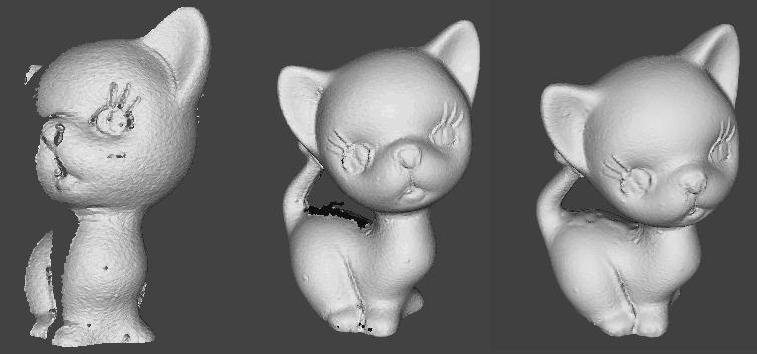
\includegraphics[width=0.8\textwidth]{kitten_pipeline.jpg}
\label{fig:pipeline}
\end{figure}
\begin{itemize}
\item Many range image patches are acquired by a 3D scanner
\item Patches are aligned and merged
\item Holes are filled and the mesh is 
\colorbox{yellow}{ 
    \textcolor{red}{ 
        \textbf{ 
            smoothed
        } 
    } 
} 
\end{itemize}
\end{frame}

\begin{frame}{Remove noise from 3D scaners}{}
  % - A title should summarize the slide in an understandable fashion
  %   for anyone how does not follow everything on the slide itself.
\begin{itemize}
\item Idea: Diffuse high curvature region by averaging over its neighborhood.
\item Problem: Remove noise without removing sharp features
\end{itemize}
\begin{figure}[htb]
\centering
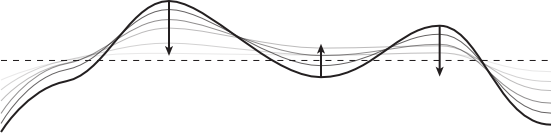
\includegraphics[width=0.8\textwidth]{ddg_heat_equation.png}
\label{fig:diffuse}
\end{figure}
\begin{figure}[htb]
\centering
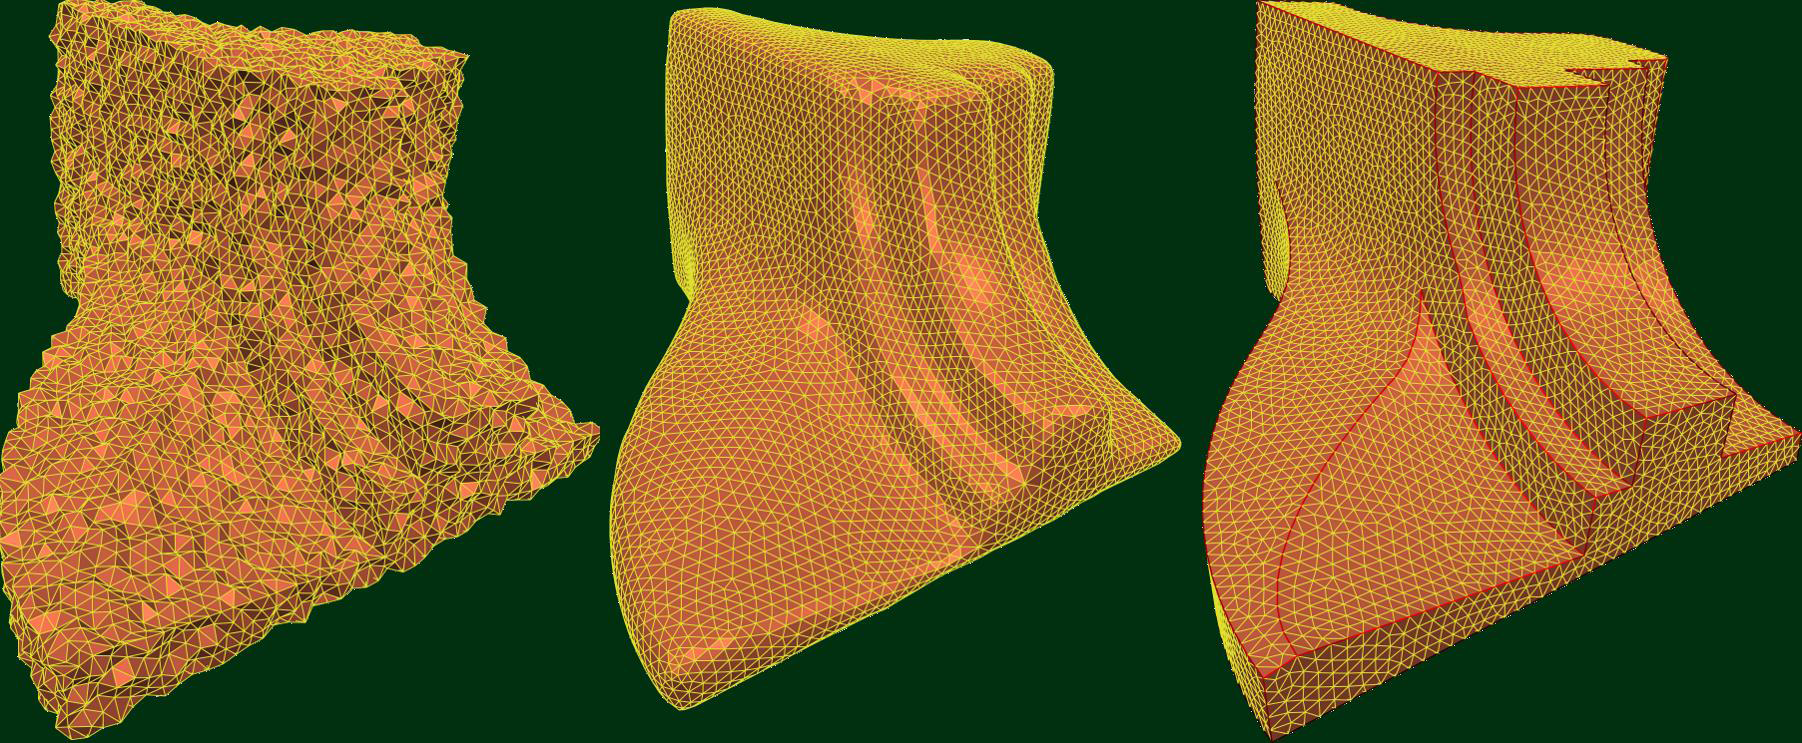
\includegraphics[width=0.5\textwidth]{motivation.PNG}
\label{fig:motivation}
\end{figure}
\end{frame}

\begin{frame}{Why Anisotropic?}
\begin{columns}
\begin{column}{0.5\textwidth}
\begin{itemize}
\item Isotropic mean curvature e.g. squared Laplacian with cotangent weight: low pass filter, sharp features not preserved. (bottom left)
\item Anisotropic mean curvature: feature detection and avoid smoothing sharp features. (bottom right)
\end{itemize}
\end{column}
\begin{column}{0.5\textwidth}
\begin{figure}[htb]
\centering
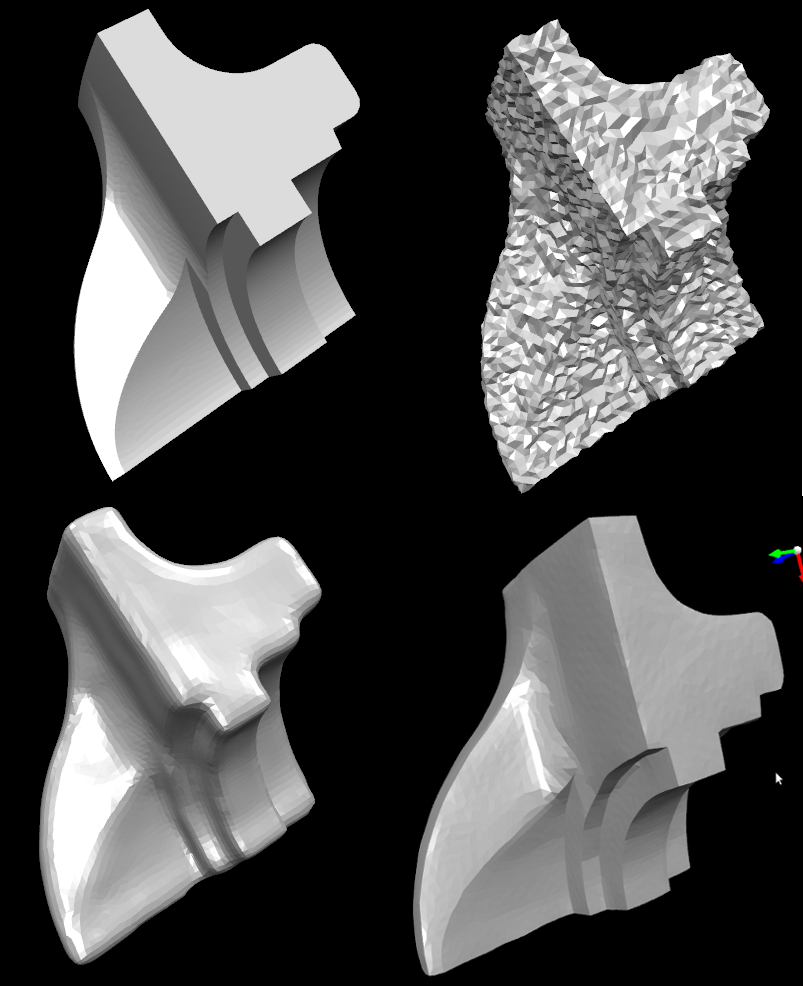
\includegraphics[width=\textwidth]{reason.png}
\label{fig:reason}
\end{figure}
\end{column}
\end{columns}
\end{frame}

\section{Anisotropic Prescribed Mean Curvature}

\begin{frame}{Mean Curvature}
%\begin{figure}[htb]
%\centering
%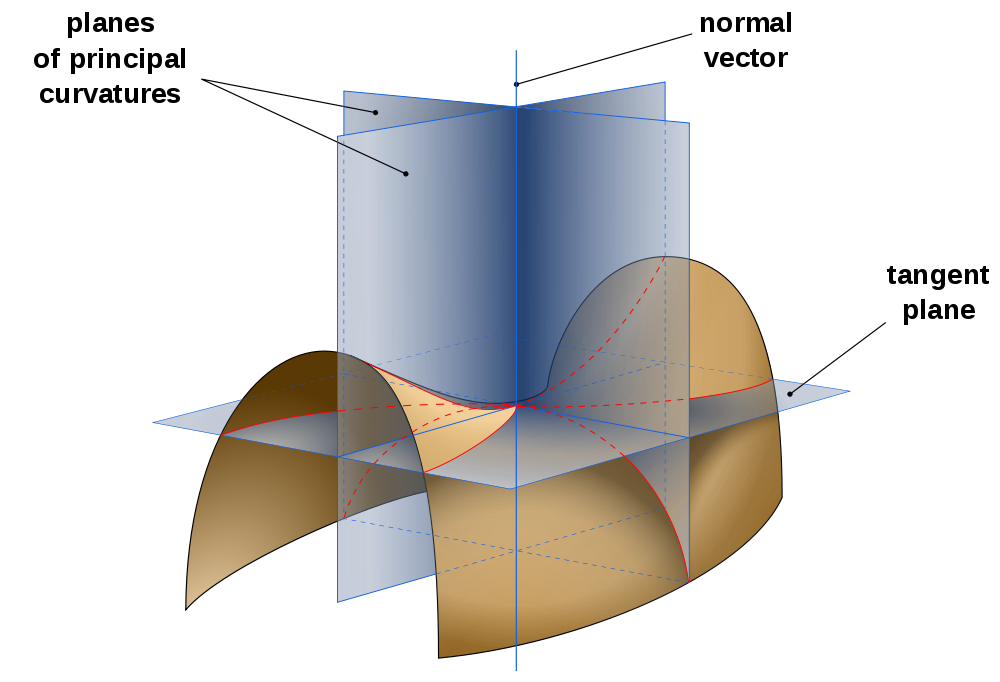
\includegraphics[width=0.4\textwidth]{principal_curvature.png}
%\label{fig:curvature}
%\end{figure}
\begin{figure}[htbp]
  \begin{minipage}[b]{0.4\linewidth}
    \centering
    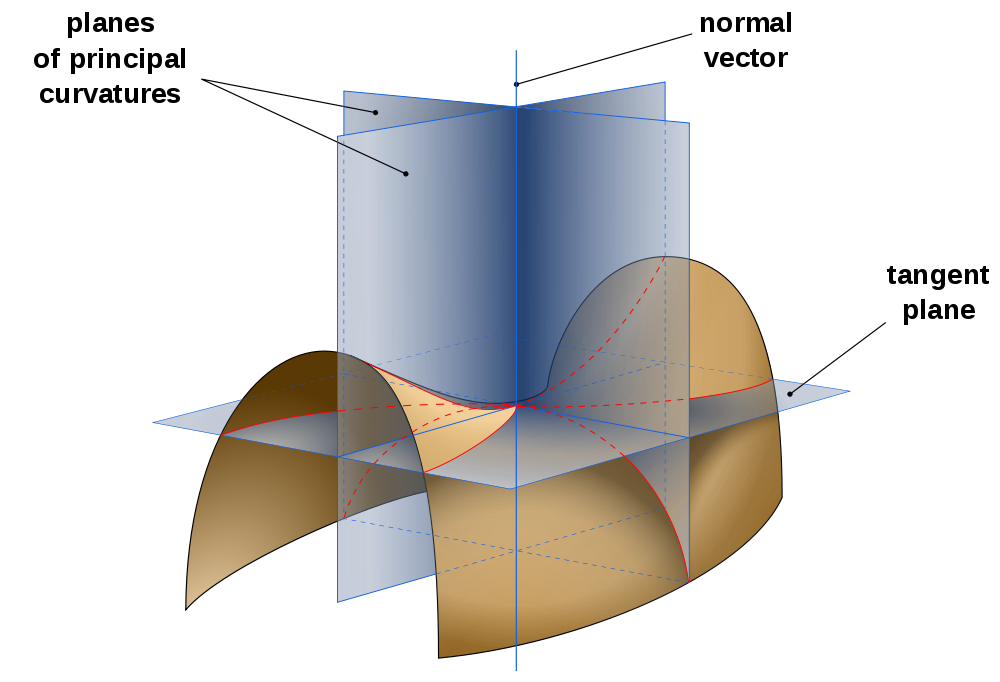
\includegraphics[width=\textwidth]{principal_curvature.png}
    \label{fig:curvature}
  \end{minipage}
  \hspace{0.5cm}
  \begin{minipage}[b]{0.4\linewidth}
    \centering
    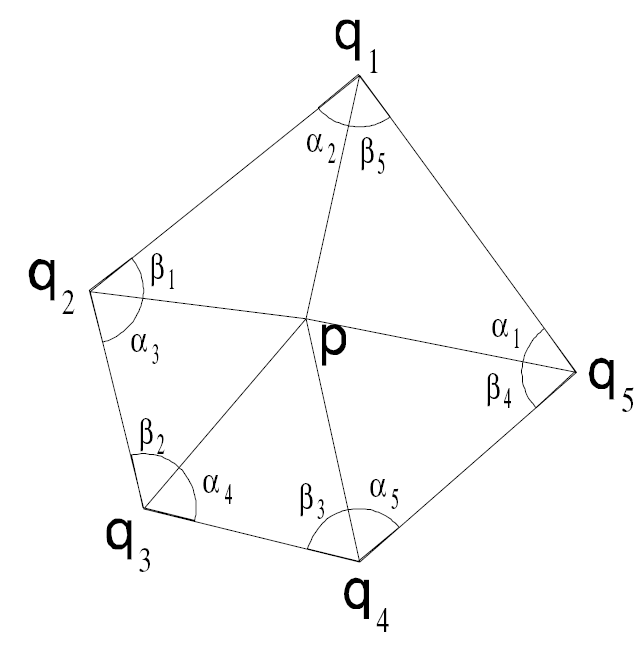
\includegraphics[width=0.6\textwidth]{cotangent.png}
    \label{fig:cotangent}
  \end{minipage}
\end{figure}
\begin{itemize}
	\item Curvature: measure deviation from flat
	\item Mean Curvature: average between min and max curvatures
	\item Smooth: reduce curvature (equivalent to area gradient)
\end{itemize}
\begin{equation*}
\bigtriangledown_p\ area\ M = \vec{H}(p) = 1/2\sum\limits_{q_i\ \in\ link\ p}{(cot\alpha_{i} + cot\beta_{i})(p-q_i)}
\end{equation*}
\end{frame}

\begin{frame}{Mean Curvature}
\begin{figure}[htb]
\centering
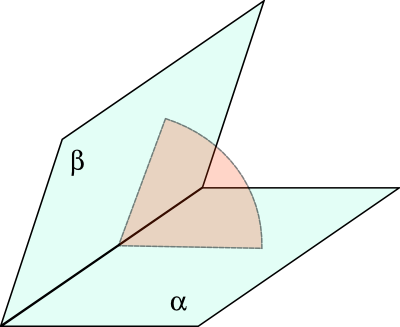
\includegraphics[width=0.25\textwidth]{Dihedral_angle.png}
\caption{Dihedral angle $\theta_e$}
\label{fig:dihedral}
\end{figure}
\begin{itemize}
	\item Let $\vec{H}(e) = H_e \vec{N}_e$ be an edge mean curvature vector, where $\vec{N}_e$ is edge normal and $H_e = 2|e|cos(\theta_e/2)$ then:
\end{itemize}
\begin{equation*}
\vec{H}(p) = 1/2\sum\limits_{e=(p, q), q \in link\ p}{\vec{H}(e)}
\end{equation*}
\end{frame}

\begin{frame}{Anisotropic Mean Curvature}
\begin{itemize}
	\item Weight less for feature vertices to avoid smoothing sharp features
\end{itemize}
\begin{equation*}
\vec{H_A}(p) = 1/2\sum\limits_{e=pq, q \in link\ p}{w(H_e)H_e \vec{N}(e)}
\end{equation*}
\begin{equation*}
w_{\lambda, r}(a) = 
\begin{cases}
1 & \text{for } |a| \leq \lambda \\
\dfrac{\lambda^2}{r(\lambda - |a|)^2+\lambda^2} & \text{for } |a| > \lambda
\end{cases}
\end{equation*}
\end{frame}

\begin{frame}{Anisotropic mean curvature flow}
\begin{itemize}
\item Explicit iteration step of the anisotropic mean curvature flow
\end{itemize}
\begin{equation*}
p^{j+1} = p^{j} - \dfrac{3s}{area(star\ p^j)}\vec{H_A}(p^j)
\end{equation*}
\begin{itemize}
\item s controls the speed of an integration step
\item Matrix form:
\end{itemize}
\begin{equation*}
\mathcal{P}^{j+1} = \mathcal{P}^j -sM^{-1}\vec{H_A}(\mathcal{P}^j)
\end{equation*}
\begin{equation*}
M_{pq} = 
\begin{cases} \dfrac{1}{6}area(star\ p), & \mbox{if } p=q \\ 
\dfrac{1}{12}area(star\ e), & \mbox{if there is an edge } e=(p, q) \\
0, & \mbox{otherwise} \end{cases}
\end{equation*}
\end{frame}

\begin{frame}{Anisotropic mean curvature - Matrix form}
\begin{figure}[htb]
\centering
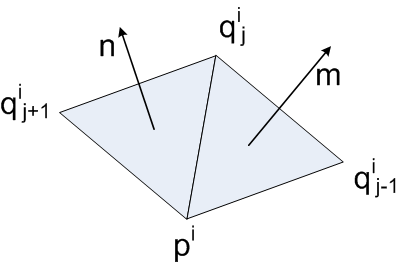
\includegraphics[width=0.35\textwidth]{edge_normal.png}
\label{fig:normal}
\end{figure}
{\small
\begin{equation*}
\begin{array} {lcl} 
\vec{H_A}(p^i) & = & 1/2\sum\limits_{q_j^i \in N(p^i)}{w(H_{e_j})H_{e_j}\dfrac{1}{\|\mathbf{n}+\mathbf{m}\|}}(\mathbf{n}+\mathbf{m}) \\ 
			   & = & \sum\limits_{q_j^i \in N(p^i)}{w_j\left[ (q_j^i-p^i)\times (q^i_{j+1} - p^i) + (q^i_{j-1}-p^i) \times (q^i_j-p^i) \right] } \\
			   & = & \sum\limits_{q_j^i \in N(p^i)}{w_j\left[ (q_j^i-p^i)\times (q^i_{j+1} - q^i_{j-1}) \right] } \\
			   & = & \sum\limits_{q_j^i \in N(p^i)}{w_j\left[ A_{\times} \cdot q^i_{j+1} - A_{\times} \cdot q^i_{j-1} \right] } \\
\end{array}
\end{equation*}
}
\end{frame}

\begin{frame}{Put them all togehter}
\begin{itemize}
\item sparse global matrix containing blocks of $3 \times 3$ cross matrices
\item row index corresponds to each one-ring center $p^i$
\item column index corresponds to a one-ring neighbor $q^i_j$
\end{itemize}
\begin{equation*}
\vec{H_A}( \mathcal{P}^i ) = 
\begin{bmatrix} 
 \cdots & \cdots & \cdots \\
 \sum\limits_{q_j^i \in N(p^i)}{w_j A_{\times}} & \cdots & -\sum\limits_{q_j^i \in N(p^i)}{w_j A_{\times}} \\
 \cdots & \cdots & \cdots 
\end{bmatrix}_{3n \times 3n} \cdot
\left[ \begin{array}{c} 
q^i_{j+1} \\ 
\vdots \\ 
q^i_{j-1} \end{array} \right]_{3n}
\end{equation*}
\end{frame}

\begin{frame}{Prescribed Mean Curvature}
\begin{itemize}
\item Energy minimization. AMC: $\vec{H_A}(p) \rightarrow 0$, APMC: $\vec{H_A}(p) \rightarrow H\vec{V_A}(p)$, where $H$ is some constant mean curvature
\item compute mean curvature ($H$), smooth this scalar field
\item evolve the surface towards a surface having this smoothed mean curvature
\begin{equation*}
p^{j+1} = p^{j} - \dfrac{3s}{area(star\ p^j)}(\vec{H_A}(p^j) - f(p^j)\vec{V_A}(p^j))
\end{equation*}
\item $f$ is a function, that prescribes the anisotropic mean curvature
\item $\vec{V_A}$ is an anisotropic volume gradient.
\end{itemize}
\end{frame}

%\begin{frame}
%\begin{itemize}
%\end{itemize}
%\end{frame}

\section{Evaluation and Results}

\begin{frame}{Evaluation}
\begin{itemize}
\item Anisotropic Mean Curvature: slow down the smoothing process in regions with high curvature, causing deformations of the surface (left)
\item Prescribed mean curvature: evolve the surface to the precomputed, smoothed mean curvature (right)
\item Matrix forms converge faster and give best results.
\end{itemize}
\begin{figure}[htb]
\centering
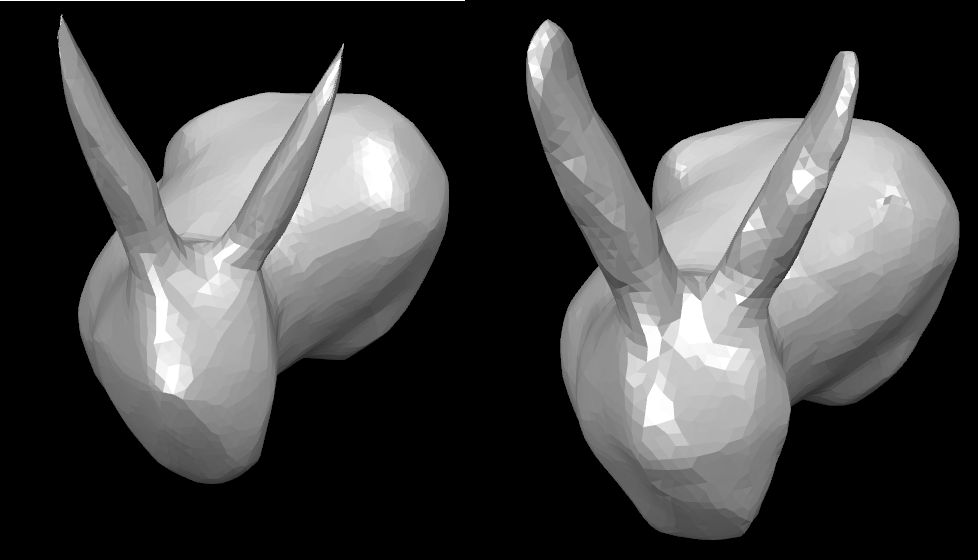
\includegraphics[width=0.5\textwidth]{amc_pmc.png}
\label{fig:amc_pmc}
\end{figure}
\end{frame}

\begin{frame}{Results}
\begin{figure}[htb]
\centering
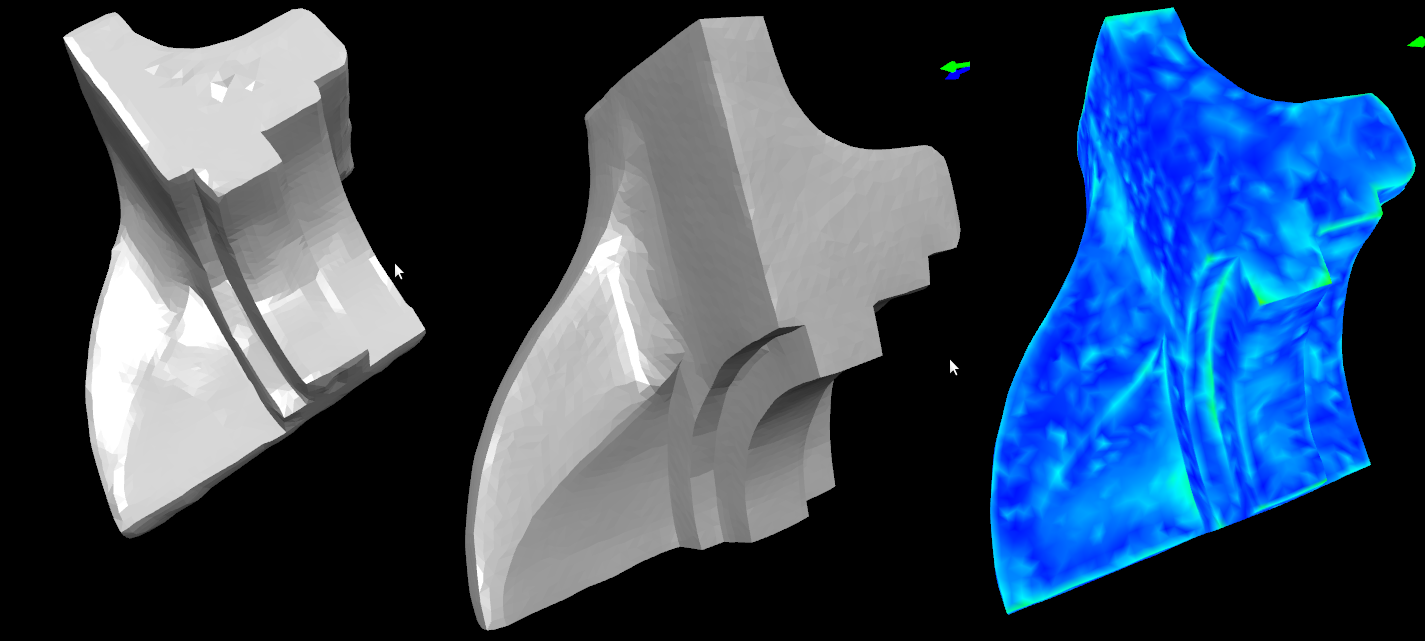
\includegraphics[width=0.9\textwidth]{results.png}
\caption{individual vertex update, batch update, color coding}
\label{fig:results}
\end{figure}
\end{frame}

\begin{frame}{Future work}
\begin{itemize}
	\item Implement implicit integration methods
	\item Extend to process boundaries
\end{itemize}
\end{frame}

\begin{frame}{Demo}
\end{frame}

% All of the following is optional and typically not needed. 
%\appendix
%\section<presentation>*{\appendixname}
%\subsection<presentation>*{For Further Reading}

%\begin{frame}[allowframebreaks]
%  \frametitle<presentation>{For Further Reading}
    
%  \begin{thebibliography}{10}
    
%  \beamertemplatebookbibitems
  % Start with overview books.

%  \bibitem{Author1990}
%    A.~Author.
%    \newblock {\em Handbook of Everything}.
%    \newblock Some Press, 1990.
 
    
%  \beamertemplatearticlebibitems
  % Followed by interesting articles. Keep the list short. 

%  \bibitem{Someone2000}
%    S.~Someone.
%    \newblock On this and that.
%    \newblock {\em Journal of This and That}, 2(1):50--100,
%    2000.
%  \end{thebibliography}
%\end{frame}

\end{document}


